\chapter*{Acknowledgments}\label{C:ack} 
Thank you Danny B for being great :- ) 

Thank you ECS Techs for putting up with my questions 

And thank you to my wonderful girlfriend for not kicking me out when I was working on this stupid fucking project really late 


% \chapter{Project Proposal}\label{A:proposal}

% % Include the entire project proposal document
% 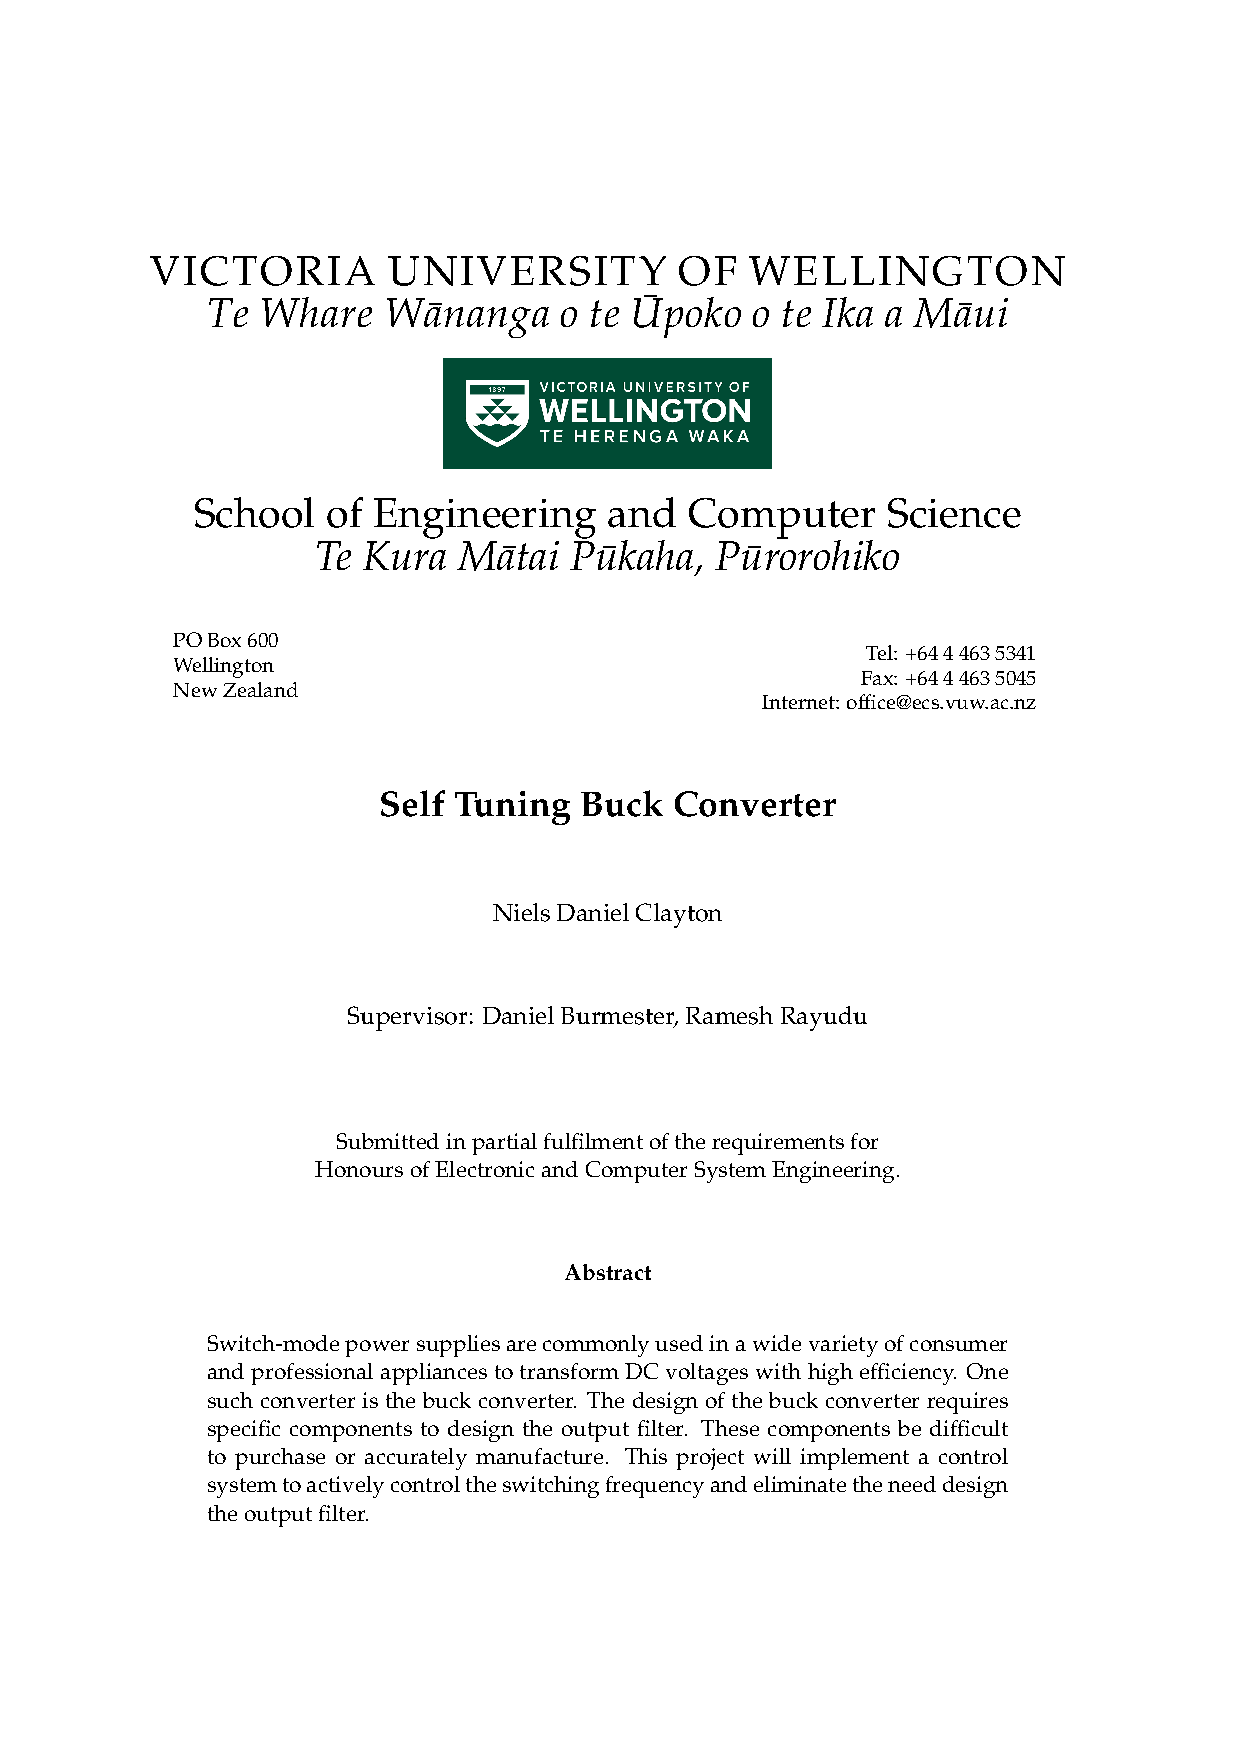
\includepdf[pages=-]{../Project\ Proposal/proj_proposal.pdf}


\chapter{System Specification Derivation Equations} \label{A:specs}

The system specification derivation equations have been input into the graphing platform \url{Desmos.com}. This has allowed me to visually inspect these equations and form conclusions. The full working and step by step derivation is also available on \url{Desmos.com} using the following links.\\

Duty cycle equation derivation:\\
\url{https://www.desmos.com/calculator/8c7wmbyzw4}\\

Inductor sizing equation derivation:\\ 
\url{https://www.desmos.com/calculator/v7ntrescw5}\\

PWM frequency equation derivation:\\ 
\url{https://www.desmos.com/calculator/ekjhcrt9zg}\\

\chapter{Analogue PWM Generation} \label{A:analogue_PWM}


\begin{figure}[H]
    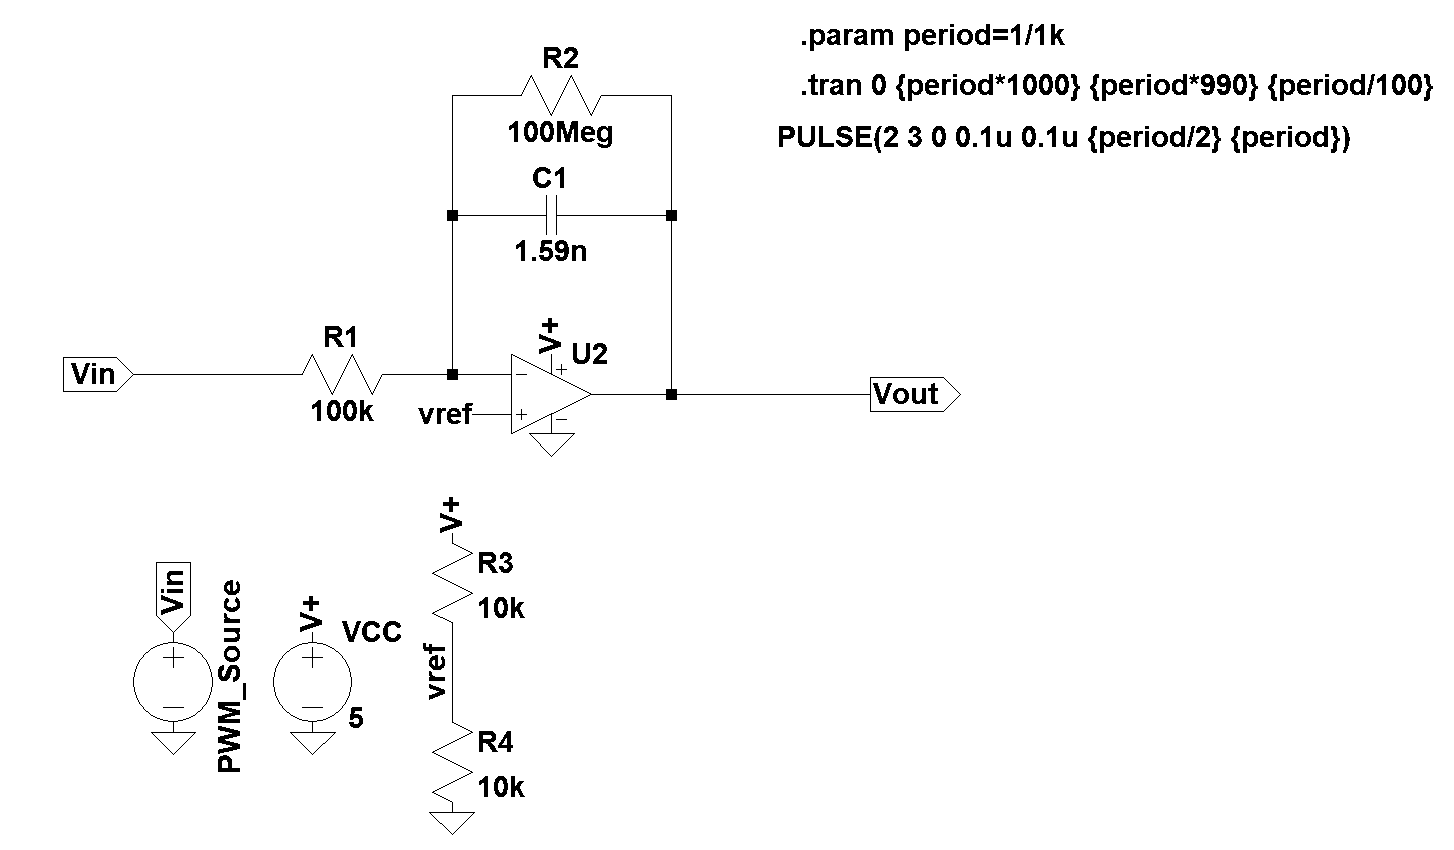
\includegraphics[width = 0.95\textwidth]{analogue_PWM_ltspice_circuit.png}
    \caption{Analogue PWM LTSpice circuit}
\end{figure}

\begin{figure}[H]
    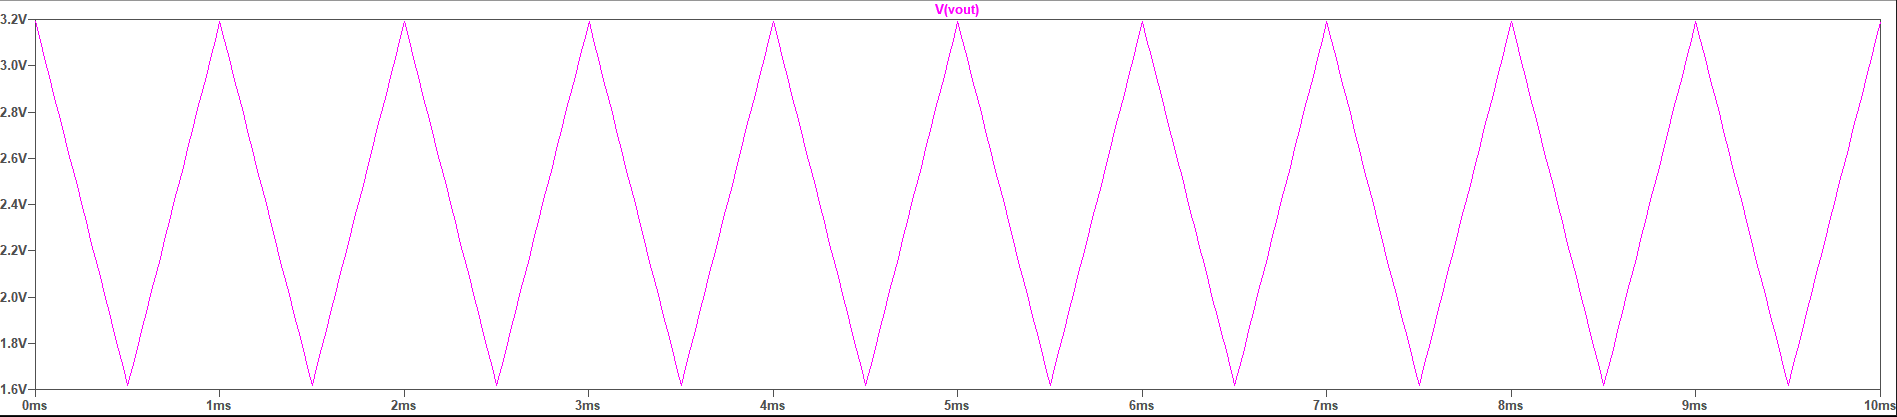
\includegraphics[width = 0.95\textwidth]{analogue_PWM_ltspice_1k.png}
    \caption{Analogue PWM LTSpice simulation 1$kHz$}
\end{figure}

\begin{figure}[H]
    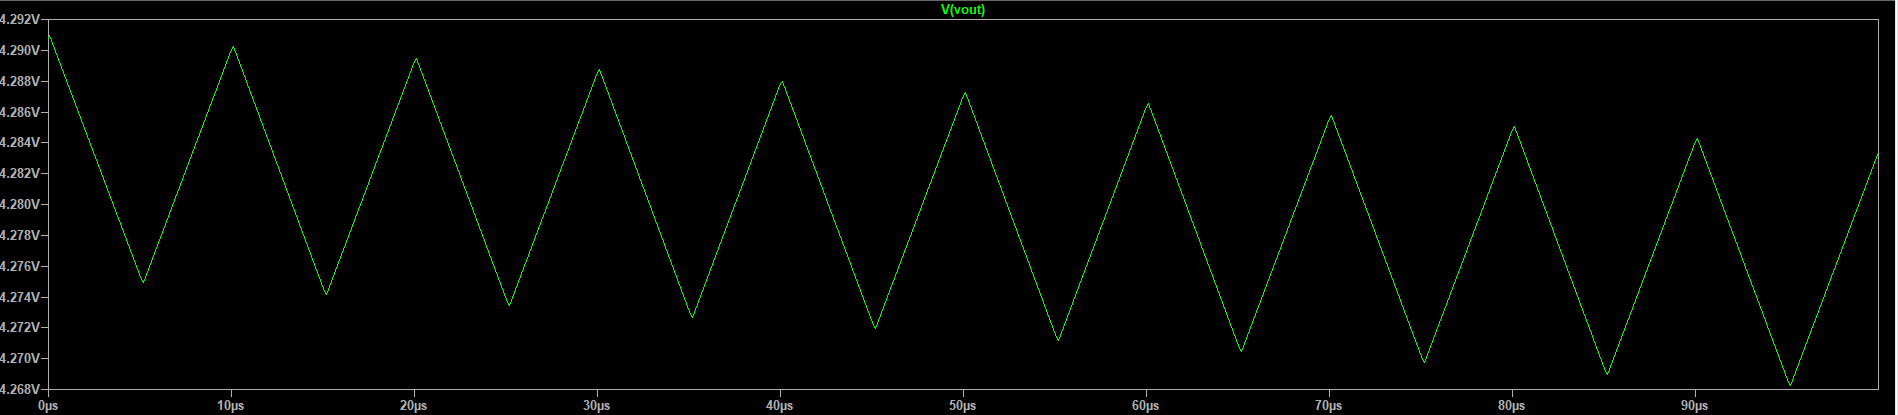
\includegraphics[width = 0.95\textwidth]{analogue_PWM_ltspice_100k.png}
    \caption{Analogue PWM LTSpice simulation 100$kHz$}
\end{figure}


\chapter{Digital PWM Generation} \label{A:digital_PWM}

\section{Digital PWM Generation Figures}

\begin{figure}[H]
    \centering
    \begin{subfigure}{0.45\textwidth}
        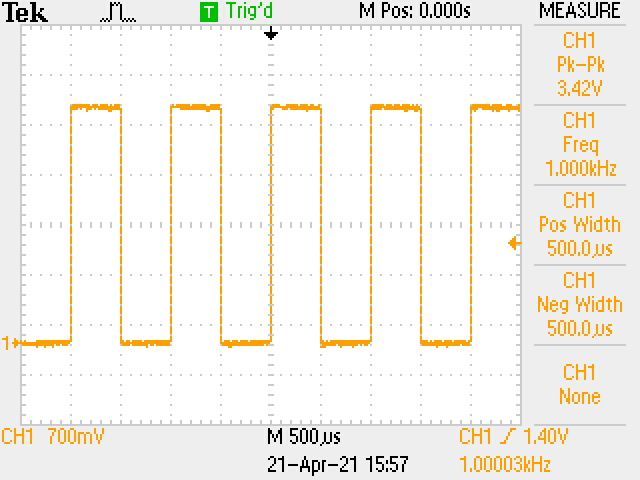
\includegraphics[width=\columnwidth]{1kHz_50Duty.JPG}
        \subcaption{Digital PWM Generation at $1kHz$ and a 50\% duty cycle}

    \end{subfigure}
    \begin{subfigure}{0.45\textwidth}
        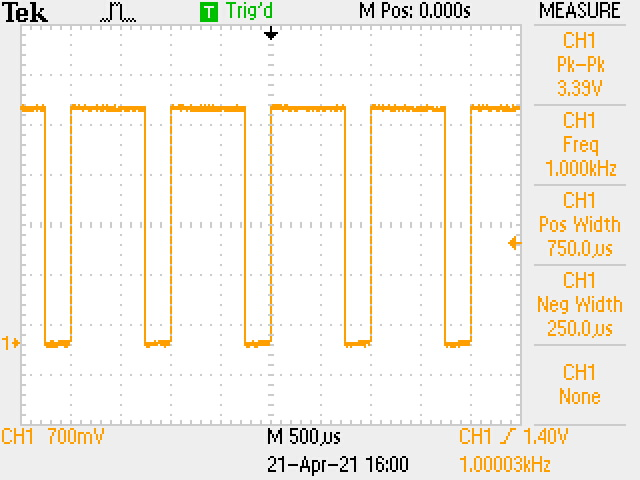
\includegraphics[width=\columnwidth]{1kHz_75Duty.JPG}
        \subcaption{Digital PWM Generation at $1kHz$ and a 75\% duty cycle}

    \end{subfigure}
    \caption{Digital PWM Generation at $1kHz$}

\end{figure}

\begin{figure}[H]
    \centering
    \begin{subfigure}{0.45\textwidth}
        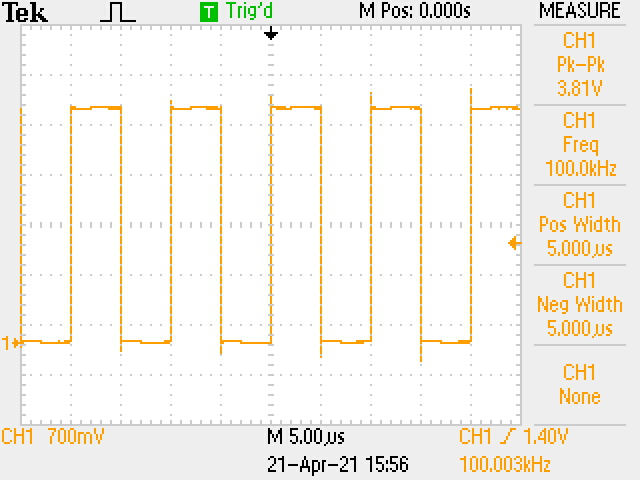
\includegraphics[width=\columnwidth]{100kHz_50Duty.JPG}
        \subcaption{Digital PWM Generation at $100kHz$ and a 50\% duty cycle}

    \end{subfigure}
    \begin{subfigure}{0.45\textwidth}
        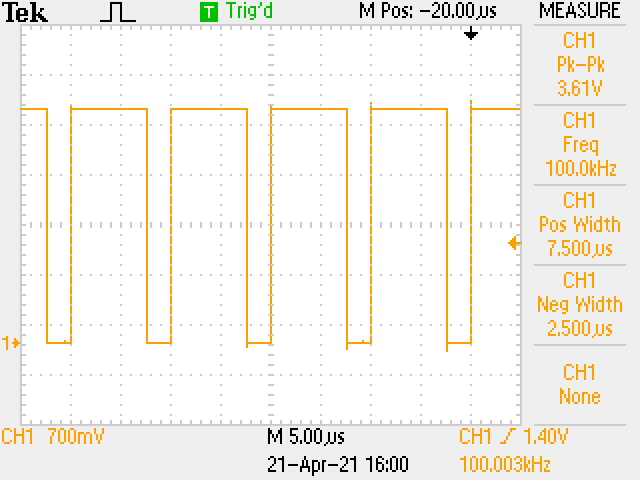
\includegraphics[width=\columnwidth]{100kHz_75Duty.JPG}
        \subcaption{Digital PWM Generation at $100kHz$ and a 75\% duty cycle}

    \end{subfigure}
    \caption{Digital PWM Generation at $100kHz$}

\end{figure}

\newpage
\section{Digital PWM Generation Code}

\lstinputlisting{code/main.c}